\documentclass[a4paper,12pt]{article}
\usepackage[francais]{babel}
\usepackage[T1]{fontenc}
\usepackage[utf8]{inputenc}
\usepackage{pslatex}
\usepackage{url}
\usepackage{graphicx}
\usepackage{lscape}
\selectlanguage{francais}


\title{Rapport de Soutenance 1}
\author{
Ihy Group : \\
deguil\_x (Xavier Deguillard)\\
genite\_n (Nicolas Geniteau)\\
sezer\_s (Stephane Sezer)\\
wagnac\_t (Teddy Wagnac)
}
\date{10 f\'evrier 2009}

\begin{document}

\maketitle

\newpage

\section*{Introduction}
Nous avons décidé cette année de nous atteler à la réalisation d'un codec audio.
L'orientation principale des projets de spé de cette année étant la recherche et
le développement, nous avons choisi de nous tourner vers les ondelettes qui
seront notre base de travail. En effet, les ondelettes étant un outil
mathématique relativement récent (elles datent du XXème siècle), elles ne sont
pas encore largement utilisées.  Il existe actuellement certains algorithmes de
compression vidéo, par exemple Dirac, leur implémentation par la BBC, mais rien
de probant pour le traitement du signal audio.\\
Notre nouveau codec révolutionnaire (du moins nous l'espérons) se nomme donc
ihy, pour deux raisons. Premièrement parce qu'``ihy'' est le nom d'un dieu
égyptien de la musique, et deuxièmement parce que ce mot est compliqué à
prononcer.\\
Ceci étant dit, entrons dans le vif du sujet. Nous présenterons dans ce rapport
le travail accompli depuis la validation du cahier des charges, les problèmes
rencontrés et leurs solutions, ainsi que le travail à accomplir pour la
prochaine soutenance.

\newpage

\tableofcontents

\newpage

\section{Travail accompli}

	\subsection{Spécifications du format ihy}
La création d'un nouveau codec passe entre autres par l'écriture des
spécifications du format. Le ihy n'échappe donc pas à la règle.\\
Chaque fichier
ihy contient un header composé des quatre lettres SNXT qui sont le FourCC
des fichiers ihy, la taille totale du fichier, le type de compression utilisé
(qui sera utile plus tard lorsque nous aurons plusieurs algorithmes adaptatifs),
le nombre de canaux ainsi que la fréquence.\\
Une deuxième partie contient
différents champs (Artiste, Album, Titre, Année, Genre et Commentaires) qui
servent à décrire le contenu du fichier audio.\\
Vient ensuite la section contenant les données à proprement parler. Cette
section contient une série de chunks décrits par leurs tailles et leurs données
respectives.\\
Ces spécifications suffisent actuellement à nos besoins, mais elles seront très
probablement étendues d'ici la fin de l'année.

	\subsection{Ondelettes}

        	\subsubsection{Interêt des ondelettes}

Le traitement du signal est indispensable dans de nombreux domaines. La
transformée de Fourier en est la base et est encore très utilisée.\\
Elle permet de convertir une fonction (pas forcément périodique) en somme de
fonctions trigonométriques grâce à un algorithme relativement simple. La
fonction d'origine est donc caractérisée uniquement par des coefficients correspondants à
la fréquence de chaque sinusoide ainsi que son déphasage. A partir de ceux-ci,
il est possible de retrouver exactement la fonction d'origine.\\
Ces coefficients permettent de traiter le signal. Si l'on veut par exemple
supprimer toutes les hautes frequences d'un signal, il suffit de supprimer les
coefficients correspondants à ces fréquences.\\
La transformée de Fourier s'applique très bien pour les signaux relativement simple.
En effet, si le signal d'entrée contient une irrégularité localisée, il va
falloir des coefficients importants pour les hautes fréquences et il en faudra
également d'autres à des fréquences plus faible pour compenser. On aura donc de
nombreux coefficients à cause d'une simple irrégularité très localisée. Le
problème vient du fait que la transformée de Fourier donne une information
uniquement sur les fréquences et non sur le temps. Pour palier ce problème, il
existe de nombreuses ameliorations tel que la transformée de Fourier à fenêtres
ou encore, la transformée par ondelettes que l'on utilisa dans notre projet.
Cela permet d'avoir une information à la fois sur le temps et sur la
fréquence.\\

		\subsubsection{Application sur un son}

Le principe mathématique des ondelettes est basé sur des fonctions continues
mais en informatique il est impossible de stocker un flux continu de données. On
est d'abord obligé de passer par un échantillonage du signal. Le principe doit
donc \^etre modifié pour utiliser des valeurs discr\`etes. Cela complique certains
aspects (basés sur la continuité) mais heuresement certains mathématiciens ont
trouvé des théorèmes anologues pour des valeurs discrètes. \footnote{il fallait bien que
tout leurs théorèmes soient utilisables}\\\\
Contrairement à la transformée de Fourier où l'on utilise des fonctions
sinusoidales idéalement infinies, on utilise une ``ondelette''. Il s'agit d'une
fonction définie sur un court intervalle et réspectant certaines propriétés
mathématiques. Il fallait encore choisir l'ondelette que l'on allait utliser dans
notre projet. Pour la premiere soutenance, nous nous sommes contenter de
l'ondelette de Haar, la plus simple a mettre en oeuvre. Elle est caractérisée de
la manière suivante :

$$ f(t) = \left\{\begin{array}{rcl} -1 & pour & 0 \leq t < 1/2 \\ 1 & pour & 1/2 \leq t < 1 \\ 0 & sinon & \end{array} \right.$$

Par un algorithme analogue à la transformée de Fourier, on calcule les
coefficients d'ondelette correspondants aux niveaux de détails à toutes les
échelles.\\
Prenons l'exemple d'une image car c'est ici plus représentatif qu'un signal
audio. Supposons que l'image fasse 4x4 pixels. Dans une première étape, on va
pour chaque bloc de 4 pixel calculer le pixel ``moyen'' (cela dépend de
l'ondelette utilisée) puis on va garder l'information perdu. On aura donc 3
coefficients par bloc de 4 pixels plus le pixel ``moyen''. A la fin du
traitement on aura une image de 2x2 pixels et 12 coefficients de détails
permettant de revenir à l'étape précedente. On réapplique le même traitement. Il
nous restera donc plus qu'un pixel (correspondant a la couleur ``moyenne'')
ainsi que 3 nouveaux coefficients. A l'aide du pixel moyen ainsi que des 17
coefficients (sur deux echelles différentes), il est tout à fait possible de
récuperer l'image d'origine avec un algorithme inverse.
\begin{center}
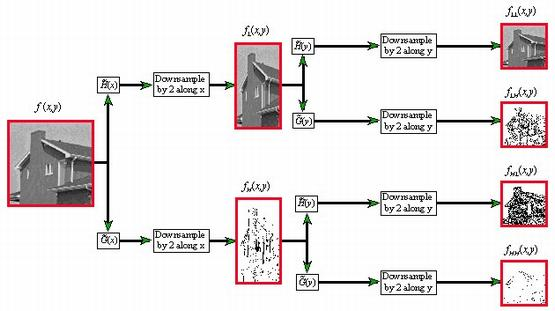
\includegraphics[scale=0.50]{img/ondelettes.jpg}
\end{center}
En applicant cet algorithme sur un signal sonore (à 1 dimenssion,
contrairement à l'exemple précedent), on obtient des tableaux de
coefficients caractérisant exactement le son d'origine. Mais ceux la
pourront être traités car ils ont un véritable ``sens''. Par exemple
les premi\`eres valeurs calculés correspondent aux hautes frequences en
fonction du temps (deux valeurs que l'on ne pouvait avoir en meme
temps avec la transformée de Fourier) alors que les derni\`eres valeurs
correspondent plus a des changements beaucoup plus lent. Avec ces
informations multi-echelles ou multi-résolutions, il sera possible de
réellement commencer la compression (avec perte) du signal audio.


	\subsection{Interfaçage Caml/C}
Les ondelettes étant faites en Caml, et l'écriture ainsi que divers
autres traitements
réalisés en C, il nous fallait faire transiter des données entre le C et le
Caml. Il y eut plusieurs étapes, envoi de données simple au Caml, puis envoi
de données plus complexe et enfin récupération de ces données.\\

		\subsubsection{Envois de données simple}
Il s'agissait de la première étape, pour comprendre comment on devait pour
interfacer le C et le Caml. Notre premier programme fût un simple envoi de
chaine de caractères, et affichage dans la console de celle-ci.\\
Le plus dur fût de trouver comment envoyer celle-ci a Caml. Pour cela, il
fallu avant tout déclarer la fonction Caml comme étant utilisable via un
``callback'' :
\begin{verbatim}
let _ =
 Callback.register "print_string" print
\end{verbatim}
Comme vous pouvez le voir, rien de bien difficile à mettre en place,
``print\_string'' était l'identifiant extérieur de la fonction Caml ``print''.
La fonction ``print'' était désormais utilisable de l'extérieur.\\
Il fallait apr\'e pouvoir l'utiliser à partir du C. Heureusement Caml fournit
des fonctions pour nous aider. Notamment les fonctions :
\begin{verbatim}
CAMLextern value *caml_named_value (char const *name);
CAMLextern value caml_callback (value closure, value arg);
\end{verbatim}
La première renvoie un pointeur sur la fonction Caml correspondant \`a ``name'',
la seconde appelle la fonction ``closure'' avec comme paramètre ``arg''. Mais
avant de pouvoir utiliser ces fonction, il fallut ``initialiser'' Caml, à
l'aide de la fonction ``caml\_main'', indispensable pour pouvoir exécuter du
code Caml.\\
La dernière chose à faire avant de pouvoir appeler le Caml était de transformer
les types C en type Caml. Cela est géré par le type ``value'' et les fonctions
associées. Après cela, la chaine de caractères était bien affichée par Caml.\\
Comme on peut le voir, la mise en place de l'interface du coté Caml est bien
plus simple que du coté du C.\\

		\subsubsection{Envois et récupération de données complexes}
Maintenant que nous pouvions envoyer une cha\^ine de caractère, il fallait essayer
d'envoyer des données plus intéressantes pour nous, c'est-à-dire un tableau de
données. Les ``ennuis'' commencèrent. Premièrement, le type ``array'' de Caml
n'est pas compatible avec les tableaux de C, il nous fallut utiliser le module
``Bigarray'' de Caml, qui lui est compatible avec les tableaux du C (il fallait
néanmoins convertir ces derniers en ``value''). Deuxièmement, dès que l'on
touchait au tableau du coté de Caml, le programme avait une ``segmentation
fault'', plutôt gênant\ldots En fait, dans le cas des entiers (plus précisément,
de tout sauf des nombres flottants), Caml les code sur 31bits (sur une
architecture 32bits) et non pas sur 32bits comme le C, il y avait donc un soucis
à l'écriture. Il fallait donc utiliser le type ``Int32'' de Caml pour modifier
le contenu du tableau, le code devient très moche et quasi illisible.
Heureusement pour nous, les ondelettes travaillent sur des nombres flottants qui
est codé de la même façon en C et en Caml.\\
Nous pouvions désormais envoyer des tableaux de flottants à Caml, et Caml
pouvait modifier à sa guise le contenu du tableau. Étape suivante : récupérer le
tableau modifié. Pour cela, rien de bien compliqué, la fonction
``caml\_callback'' vue précédemment nous renvoie sous forme de ``value'' le
résultat de la fonction appelée. Il suffisait désormais de récupérer le tableau
contenu dans le ``value'', et encore une fois Caml fournit une fonction (ou
plutôt une macro ici) : ``Data\_bigarray\_val'' qui renvoit le tableau contenu
dans un ``value'' représentant un ``bigarray''.

	\subsection{Algorithme de Huffman}
Algorithme extrêmement utilisé dans le monde de la compression, il doit sa
popularité à son efficacité quelques soit le type de données à compresser. Son
principe est simple, un caractère classique est codé sur un octet ou huit bits,
Huffman considère que les caractères les plus fréquents doivent être codés avec
le moins de bits possible.\\
Dans la pratique, il faut créer ce qu'on appelle un arbre de Huffman, qui est un
arbre binaire localement complet (chaque noeud a soit deux fils soit aucun),
non équilibré, les caractères sont dans les feuilles de l'arbre et leur nouveau
codage est tout simplement est leur représentation par occurence (on ajoute un 1
a droite du code lorsqu'on part à droite et un 0 lorsqu'on part à gauche, tout
ceci de façon récursive).\\
Au niveau implémentation, il nous a fallu procéder à un comptage des occurrences
de chaque caractère, puis création d'une file de prioritées, implémentée grâce à
un tas, ce qui nous assure un ajout et un retrait en temps logarithmique.
Lorsque la file de prioritées est créee, il nous faut ensuite construire l'arbre
en tant que tel. Cela se passe en plusieurs étapes :
\begin{enumerate}
\item tant qu'il y a plus d'un élément dans la file :
\begin{enumerate}
\item récupérer les deux élements de plus haute priorité (fréquence la
plus basse).
\item créer un noeud qui a pour fils les deux élements précédent et qui
a pour fréquence la somme des fr\'equences de ses deux fils.
\item ajouter ce noeud à la file
\end{enumerate}
\item le dernier noeud est la racine de l'arbre d'Huffman
\end{enumerate}
À partir de cet arbre, on peut déterminer le nouveau codage de chaque caractère,
à l'aide d'un simple parcours profondeur de l'arbre, et à partir du nouveau
codage, on peut déterminer le nouveau fichier compressé.\\
Nous devions régler un dernier soucis : comment lors de la décompression
récupérer le flux original? Il suffit dans la théorie de stocker l'arbre de
Huffman, ou du moins suffisamment de données pour pouvoir le retrouver. La
technique employée ici est assez simple (et peut-être pas optimale) et a le
mérite de marcher. Chaque nœud de l'arbre sera codé sur 2 octets, un octet
indiquant s'il s'agit d'une feuille ou d'un nœud internet, le second octet sert
uniquement pour les feuilles, il indique le caractère correspondant à la
feuille. Ces informations sont écrites suivant leur ordre d'un parcours largeur,
on peut ainsi facilement détecter les changements de niveaux lors de la
décompression.\\
Nous avons réalisé quelques tests, pour évaluer la capacité pour Huffman de
compresser des données. Sur la musique Black Sabbath du groupe éponyme, qui fait
66méga-octets en wav, après passage dans l'algorithme de Huffman, celle-ci ne
fait plus que 55méga-octets, soit 11méga-octets, ou en terme de pourcentage, un
peu moins de 20\%. En sommes, plutôt intéressant.\\

	\subsection{Lecture de son}
La lecture du son, un indispensable lors de la création d'un codec audio, pour
au moins comparer le morceaux initial et celui compressé.\\ Pour cela nous
utilisons une bibliothèque extrêmement simple : libao.  Elle est de plus multi
plateformes et fonctionne donc sur tous les UNIX.  Son fonctionnement est
simple, on récupère le ``device'' audio, correspondant à la sortie audio de
l'ordinateur, puis on indique la taille d'un échantillon, sa fréquence
d'échantillonnage, le nombre de canal\ldots, tout ce qui est nécessaire à la
lecture d'un son. Puis on construit un tableau de caractère, qui est identique
dans sa structure que les données dans un fichier wav, et on peut le jouer. Tout
ça grâce à ces trois fonctions :
\newpage
\begin{verbatim}
void ao_initialize(void);
ao_device* ao_open_live(int driver_id,
 ao_sample_format *format,
 ao_option *option);
int ao_play(ao_device *device,
 char *output_samples,
 uint_32 num_bytes);
\end{verbatim}
Qui servent respectivement à : initialiser le système, ouvrir la carte son pour
pouvoir y lire de la musique, et finalement, lire du son. Rien de plus simple,
bien sur cela impose d'avoir le ``output\_samples'' correctement formé.\\
Grâce à cela, on peut lire un fichier wav sans problèmes, la lecture d'un
fichier ihy n'étant pas encore opérationnelle.\\

	\subsection{Premières étapes de threading}
De nos jours, les processeurs ont de plus de plus de cœurs, ils peuvent donc
exécuter de plus en plus de tâches simultanément, et donc faire des traitements
plus rapides si cette exécution simultanée est bien pensée.\\
La compression audio est particulièrement bien adaptée à cette exécution
simultanée, dites ``concurrentielle''. En effet la compression d'une partie de
la musique ne dépend pas du résultat d'une partie précédente (dans notre cas).
On peut donc mettre en place des ``threads'', un thread permettant cette
execution simultanée au sein d'un même programme, chaque thread calculant une
partie de la musique. Dans la pratique, un thread ne calcule pas uniquement une
partie mais plusieurs petites parties, ceci pour réduire encore la durée d'un
traitement.  Pour illustrer cela, prenons un exemple : utilisons 2 threads et
considérons que la première partie de la musique met deux fois plus de temps que
la deuxième partie. Le premier thread va compresser la première partie, et le
deuxième la deuxième, comme on peut s'en douter, le deuxième thread mettre deux
fois moins de temps pour finir et sera inactif pendant le reste de la
compression.\\
Pour pallier à ce problème, il faut découper la musique en un certain nombre de
morceaux, puis écrire une fonction qui va permettre a un thread de récupérer le
prochain morceau à calculer. Cette fonction doit bien évidement être
``thread-safe'', c'est-à-dire que si elle est appelée au même moment par
plusieurs threads, elle ne doit pas renvoyer deux fois le même morceaux à
calculer, ou avoir un comportement indéfini. Ceci est réalisé en utilisant ce
que l'on appelle des ``mutex'', un mutex possède deux états : libre ou bloqué.
Lorsqu'un thread tente de bloquer un mutex déjà bloqué, il attend jusqu'à ce que
ce dernier devienne libre. Leur utilisation dans notre cas devient alors assez
évidente. Lorsque la fonction est appelée, un mutex est bloqué et est libéré
lorsque la fonction se termine, assurant ainsi le ``thread-safe''.\\
On pouvait désormais compresser une musique de façon parallèle. Une autre
utilisation, totalement différente cette fois-ci, était de pouvoir lire la
musique alors que l'on compressait les données. On a alors deux threads,
totalement séparés, un thread jouant de la musique, et un autre compressant
cette même musique.\\

		\subsubsection{Problèmes rencontrés}
Mais voila, tout n'est pas aussi rose dans la pratique, si la partie ``thread de
lecture et thread de compression'' fonctionne parfaitement, il n'en est pas de
même pour la partie ``multiple thread de compression''. Comme dit précédemment,
la compression est faites par Caml et Caml utilise ce que l'on appelle un
``Garbage Collector'' pour gérer la mémoire sans que l'utilisateur n'ait à se
soucier de pointeurs et autres joyeusetés du genre. Seulement ce ``Garbage
Collector'' n'est pas ``thread-safe''\footnote{voir ci-dessus}, ce qui implique
que lorsque un thread fait des calculs sur un une partie de la musique et que
l'autre réorganise la mémoire à l'aide de ce fameux ``Garbage Collector'', le
premier va soudainement vouloir écrire au mauvais endroit de la mémoire, en
résulte une ``segmentation fault'' insolvables.\\
Il y a néanmoins une solution pour résoudre ce problème, que nous avons
partiellement explorée. Il s'agit du concept de ``fork'', dans un thread
classique, chaque thread partage la même mémoire, facilitant ainsi les
manipulation de la mémoire, alors qu'un fork est tout simplement un clonage
intégral du programme. Les deux programmes ne partagent plus la même zone de
mémoire, ils sont séparés. Cela règle notre problème, mais ajoute un autre
problème, également assez génant : comment faire pour partager une zone de
mémoire? Car n'oublions pas notre but est de partager le travail sur plusieurs
coeur du processeur, non de faire deux fois le même travail. La solution se
nomme ``pipe''.  Pour le moment cela reste extrêmement théorique, et par soucis
de clarté, non implémentée.\\

\newpage

	\subsection{Ce que notre programme fait}
Pour le moment, notre programme réalise plusieurs choses. Premièrement, il lit
un fichier wav et le place en mémoire, il s'agit du premier argument de notre
programme. À partir de ce fichier wav, il le joue en arrière plan. Il applique
ensuite les ondelettes sur ce fichier et l'écrit dans un fichier passé en
deuxième paramètre. Nous appliquons ensuite l'algorithme de Huffman sur le
fichier wav et mesurons la différence entre le fichier original et le fichier
``compressé'', ceci pour évaluer la performance de cet algorithme. Puis, à
partir du fichier ihy précédemment créer, nous appliquons les ``ondelettes
inverses'' et écrivons le fichier wav ainsi obtenu dans le troisième argument du
programme.\\

	\subsection{Interface graphique en GTK}

		\subsubsection{Petite présentation de GTK+}
La bibliothèque GTK+ permet de créer des interfaces graphiques (GUI) assez
simplement. C'est pour cela que nous avons choisi cette librairie, afin de
développer une interface graphique interactive et attrayante. A l'origine, GTK+
a été développée pour donner des bases solides au logiciel de traitement
d'images GIMP (GNU Image Manipulation Program). Aujourd'hui, le domaine
d'application de cette bibliothèque ne se limite pas à GIMP : elle est utilisée
dans d'autres projets. Le développement phare est l'environnement  GNOME (GNU
Network Object Model Environment).

		\subsubsection{Notre lecteur Ihy}
Tout d'abord, avant de développer l'interface idéale il fallait nous
familiariser avec GTK et son principe de widget (Window Gadget) qui sont les
objets graphique de GTK+. Un widget est en fait une structure définissant les
propriétés d'un objet associé à une large panoplie de fonctions permettant de
manipuler ces objets. Donc, nous avons décidé de commencer en développant une
fenêtre de base qui représente notre futur lecteur audio. En effet, nous avons
une fenêtre de dimension 620x400 pouvant apparaitre à un endroit aléatoire sur
le bureau avec les trois icônes de base qui permettent de fermer, réduire et
restaurer la fenêtre. De plus, la fenêtre contient un titre « Lecteur Ihy ».  La
fenêtre contient deux box. Une Box permet d'inclure plusieurs widgets à
l'intérieur d'une fenêtre, sans ça il est strictement impossible de le faire.
Pour notre part, nous détenons 2 Box. Une Box verticale (GtkVBox) qui permet de
disposer les widgets verticalement, qui elle contient une Box horizontale
(GtkHBox) qui dispose les widgets horizontalement. La Box horizontale contient
cinq boutons. Les cinq boutons indispensable pour un lecteur audio, c'est-à-dire
PLAY, STOP, PAUSE, AVANCE et RETOUR. Chacun de ces boutons viennent du stock
direct de GTK+ qui est pour sa part plutôt vaste. Les cinq boutons sont
positionnés horizontalement comme dis précédemment, de même dimension et ce
partage l'espace équitablement selon le principe de la Box dans GTK.  Tandis
que, la Box verticale, en plus de détenir la Box horizontale, détient une barre
de progression, qui se remplit à l'aide d'un clic sur le bouton PLAY. Pour
cela, on utilise une fonction de GTK+ qui permet de faire une seul itération.
Donc à ce moment là GTK+ va reprendre la main puis la rendre aussitôt, si bien
qu’il pourra mettre à jour les widgets.  Voilà en quelques termes ce que
nous avons pour notre première ébauche.
\begin{center}
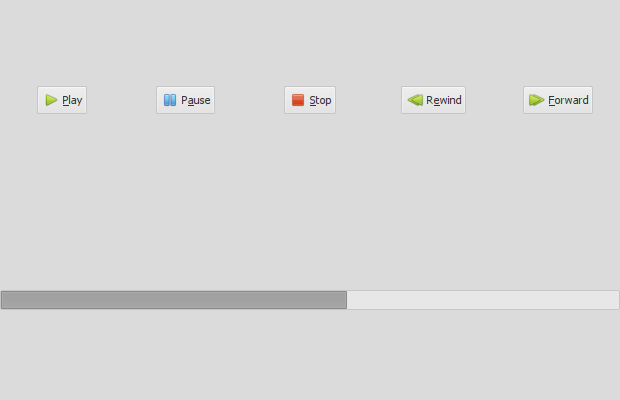
\includegraphics[scale=0.50]{img/gtk.png}
\end{center}
	\subsection{Site web}
Disponible à l'adresse suivante : \url{http://rip-rip.github.com/ihy/}, le site
web est des plus basiques, il présente succinctement le projet, les auteurs du
projet. Le projet est également téléchargeable, dans une version mise à jour
dynamiquement via deux icônes présentes en haut à droite de la page, permettant
de télécharger la dernière mise à jour du git dans le format zip ou tar.

\newpage

\section{Tâches prévues}

	\subsection{Ajout du type half}
Un des gros problèmes que nous avons actuellement réside dans le fait que la
plupart des échantillons dans un fichier pcm sont codés sur 16 bits, et qu'un
flottant, par défaut est codé sur 32 bits. Sachant que nous n'utilisons
actuellement aucune méthode d'élimination des données, nous obtenons un
fichier ihy qui fait précisément deux fois la taille du fichier pcm original
(modulo la taille des headers).\\
Il est aisé de comprendre que c'est un petit peu embêtant pour un format de
compression audio\ldots\\
Un format qui est actuellement dans un draft de la prochaine spécification
IEEE754 est le half precision floating point number. En effet, comme son nom
l'indique, ce type de données utilise 16bits pour stocker un nombre à virgule
flottante. Le résultat obtenu lors d'un traitement avec les ondelettes n'ayant
pas besoin de la précision apportée par les flottants 32bits, ce format est
farpaitement\footnote{Voir Asterix \& Obélix, les lauriers de César} adapté à nos
besoins.\\
Le souci réside dans le fait que ce format n'est ni utilisé dans les processeurs
x86 actuels (il le sera probablement avec les instructions SSE5), ni utilisable
en C. Il nous faudra donc l'implémenter nous même et écrire les fonctions de
conversions half\_to\_float et float\_to\_half correspondantes.

\newpage

	\subsection{Ondelettes}
\subsubsection{Changement d'ondelette}
Nous utilisons pour le moment l'ondelette de Haar car son
implémentation est très simple mais celle-ci n'est pas réelement
adapté au traitement d'un signal audio. En effet, il faudrait trouver
une ondelette qui engendrerait plus de coefficients nuls pour avoir
une meilleure compression. On hésite encore entre deux solutions.\\
\begin{enumerate}
\item 
  Une première solution serait de trouver une ondelette génerale qui
  donnent de bons résultats sur la plupart des signaux audios. Il va
  donc falloir en implémenter plusieurs puis faire de nombreux tests
  (qui pourront être automatisés).  
\item 
  Une autre solution serait d'analyser le signal audio et de créer
  l'ondelette la plus adaptée. Cette méthode donnerait les meilleurs
  résultats mais engendrent de nombreux problèmes. En effet, il est
  très difficile de trouver la (ou l'une des) meilleure ondelette qui
  respectent toutes les propriétés mathématiques nécessaires. De plus,
  l'algorithme actuel est optimisé pour une ondelette spécifique (ici,
  Haar) mais l'algoritme géneral a une complexité en o(N carre log N).
  Ce qui ne pourrais pas être utilisable avec un fichier son, du
  moins en temps réel. Le dernier soucis serait de trouver une façon
  de stocker dans le fichier ihy l'ondelette, qui est une fonction
  mathématique.
\end{enumerate}
\subsubsection{Traitement des coefficients, psychoacoustique}
Maintenant que l'on a tout les coefficients grâce à la transformée en
ondelette, il va falloir trouver un moyen pour réellement faire de la
compression (avec perte). Nous devrons modifier les coefficients qui
influent peu sur la perception du son par l'oreille humaine. Nous
savons par exemple que l'on peut supprimer les fréquences supérieurs à
20KHz et inférieurs à 20Hz. On peut également supprimer les fréquences
masqués (une onde avec un amplitude très élevée masque une autre onde
avec une amplitude beaucoup plus faible). Pour avoir les meilleurs
resultats, de nombreux tests et recherches seront necessaires.

\newpage

	\subsection{Threading total de la compression/décompression}
La tendence depuis quelques ann\'ees \'etant \`a la multiplication du nombre de processeurs/coeurs dans chaque machine, il serait judicieux de s'en servir pour accelerer les operations de compression decompression dans notre logiciel.\\
En effet, les compressions/decompressions sont des operations hautement parralelisables. Il suffit de creer autant de processus que de coeurs disponibles pour utiliser au maximum le processeur, et d'assigner a chaque processus un bloc de donnees a traiter. L'utilisation d'une file de priorite pour ce genre de taches est tres utile, et nous ferons probablement de meme.\\
Le seul souci sera probablement le garbage collector de caml qui s'associe mal avec les pthreads. Nous utiliserons donc des forks qui cloisonnent bien l'etendue de la memoire de chaque processus.

	\subsection{Amélioration de l'UI}
Pour la prochaine fois, nous comptons
rendre notre lecteur plus attractif et tenter de le faire paraitre plus comme un
lecteur audio. Pour cela, nous comptons utiliser des tables qui permettent dans
GTK+ de mieux placer les widgets dans les Box afin d'avoir plus de précision. \\
Nous commencerons aussi \`a nous interesser au spectrographe qui permettra d'obtenir un resultat plus interessant.
\begin{center}
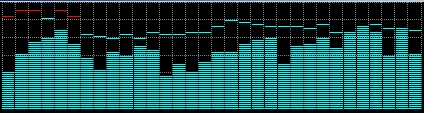
\includegraphics[scale=0.50]{img/spectre.png}
\end{center}

\newpage

\section*{Conclusion}
Comme vous pouvez le voir, le projet avance, et même plutôt bien. Nous sommes
dans les temps vis-à-vis de ce que l'on avait prévu, ce qui est une bonne chose,
vu les difficultés rencontrées ainsi que le but du projet. Rappelons le notre
projet a pour but de faire un codec concurrent au vieux MP3.\\
Il n'y a en fait qu'une seule divergence par rapport au cahier des charges, le
fait que nous n'utilisons plus svn comme gestionnaire de version, nous nous
servons désormais de git et notre projet est hébergé par github, et tout cela
marche fortement bien.\\
En ce qui concerne le groupe, rien à signaler, chacun fait ce qu'il a à faire en
temps et en heure et tout va pour le mieux.\\
``Un dernier mot pour la fin? Carotte''\footnote{merci Kamoulox}\\

\newpage

\section{Annexe}
	\subsection{Représentation graphique des coefficients d'ondellette}
En parallèle de l'éxecutable géneral, nous avons également développé
un petit programme qui, à partir d'un fichier wav, calcule les
coefficients d'ondelette et les affiche sous forme d'image.\\
Les coefficients donnent trois informations simultanéments :
l'échelle, le temps et l'amplitude. Nous avons représenter ces trois
informations sur une image en deux dimenssions de la manière suivante
: l'axe des abscisse correspond au temps, l'axe des ordonnée à
l'échelle (ici en logarithme de 2) et le degrés de gris à l'amplitude. Plus
l'amplitude est élevée, plus le niveau de gris se rapproche du noir.
Voici le résultat obtenu avec quelques secondes de musique :\\
\begin{center}
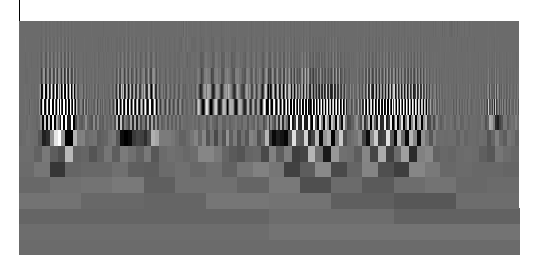
\includegraphics[scale=0.50]{img/coeffs.png}
\end{center}
Ce schéma nous apporte plusieurs informations. Tout d'abord, ce schéma
montre bien le principe d'incertitide d'Heisenberg. En effet, on
remarque que pour avoir une précision de plus en plus importante sur
la fréquence, on perd la précision sur le temps. Et inversement, pour
avoir une précision sur le temps, on perd en précision sur la
fréquence. Cela pourrait être encore plus représentatif avec une
échelle non logarithmique pour l'axe des ordonnée, mais le schéma
serait moins lisible.\\
On voit également de forts contrastes aux échelles moyennes. Cela nous
apprend qu'une majorité de l'information se trouve à ces échelles.
\\
Cette petite application devrait nous aider pour le traitement des
coefficients.
\end{document}
